\chapter{SWITCHengines}
\section{Création d'un compte sur SWITCHengines}

Toute personne qui possède un compte AAI chez SWITCH (SWITCHaai) peut créer un compte sur SWITCHengines, le cloud privé de SWITCH. Pour ce faire, il faut aller à l'adresse \url{https://cloud-id.switch.ch/}. Vous serez redirigé vers une page de connexion AAI standard (figure \ref{loginAAI}a). Il vous faudra alors sélectionner l'école dans laquelle vous êtes enregistré puis entrer votre nom d'utilisateur et mot de passe (figure \ref{loginAAI}b).

\begin{figure}[h!]
    \centering
    \begin{tabular}{cc}
      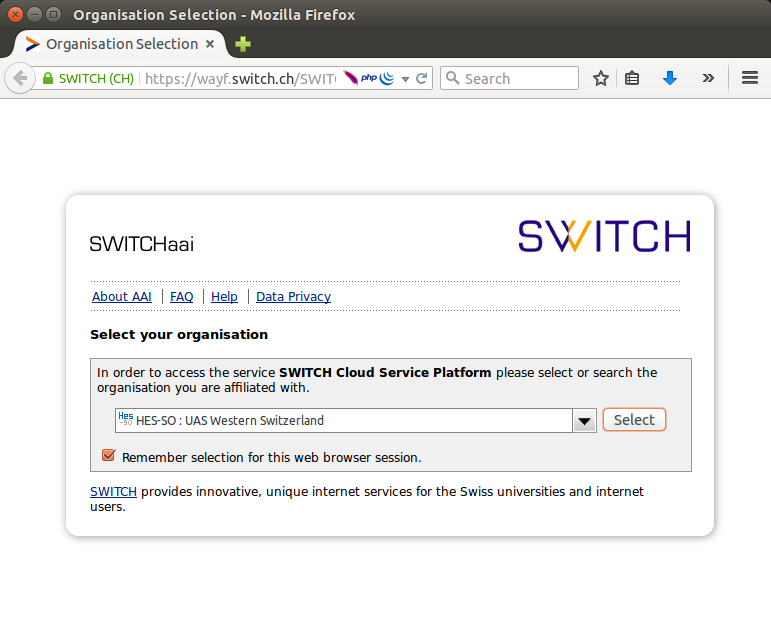
\includegraphics[width=.48\linewidth]{img/switch1.png} &
      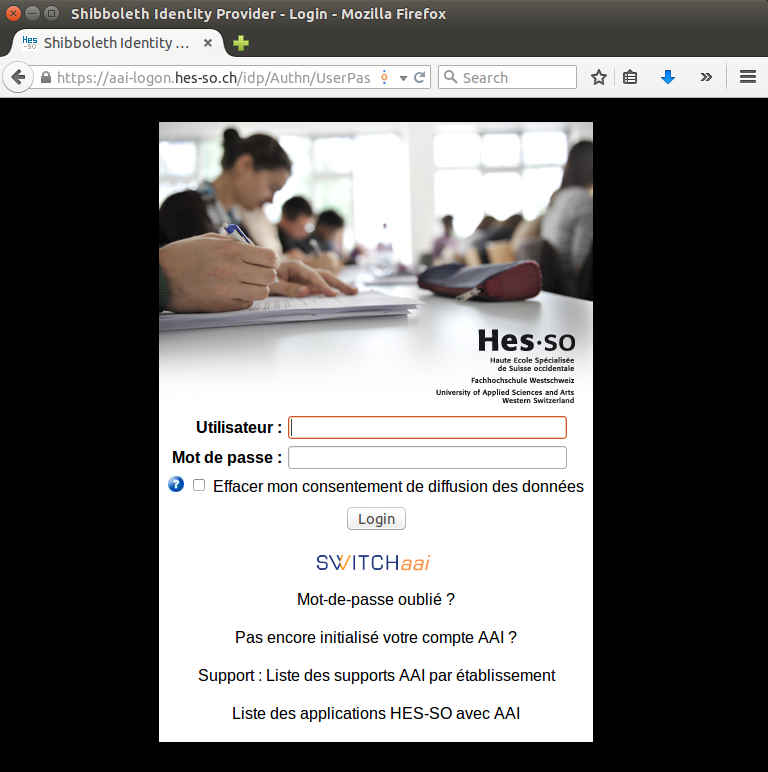
\includegraphics[width=.48\linewidth]{img/switch2.png} \\
      (a) & (b)\\
    \end{tabular}
    \caption{Connexion AAI (a) Ecole (b) Utilisateur et mot de passe
    \label{loginAAI}}
\end{figure}

Une fois connecté, vous arriverez sur une page qui vous propose de créer un compte pour pouvoir accéder au Cloud Service de SWITCH (figure \ref{loginEngines}a). Cliquez donc sur le lien prévu à cet effet. On vous demandera alors de choisir un mot de passe (figure \ref{loginEngines}b).

\begin{figure}[h!]
    \centering
    \begin{tabular}{cc}
      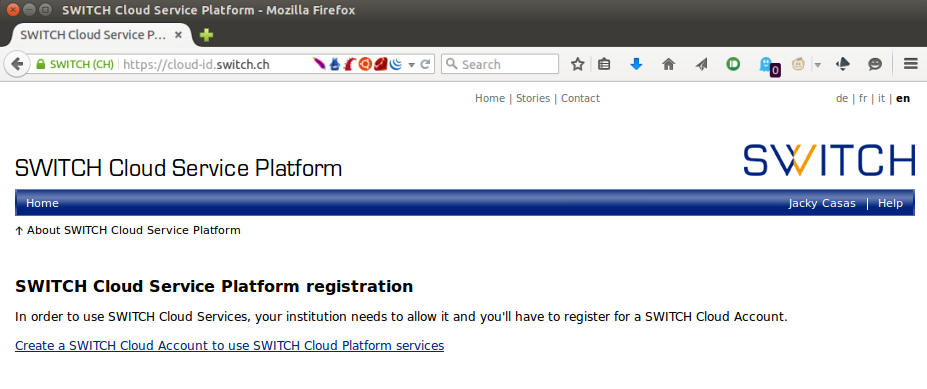
\includegraphics[width=.48\linewidth]{img/switch3.png} &
      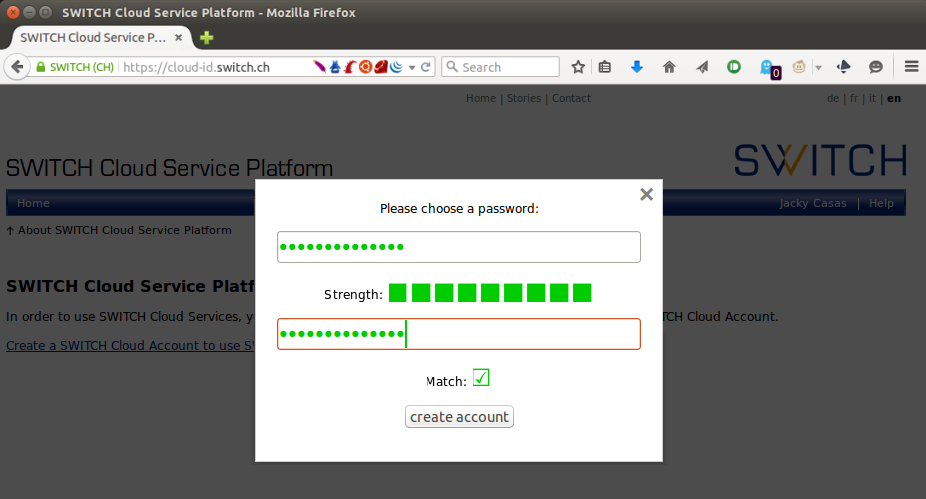
\includegraphics[width=.48\linewidth]{img/switch4.png} \\
      (a) & (b)\\
    \end{tabular}
    \caption{Création du compte Cloud Service (a) Accueil (b) Choix du mot de passe
    \label{loginEngines}}
\end{figure}

Vous arrivez ensuite sur une page récapitulative qui vous indique votre identifiant (attention, il peut être différent de votre identifiant AAI). Et en dessous vous voyez les différents services auxquels vous avez accès. Vous pouvez voir cette page à la figure \ref{enginesRecap}.

\begin{figure}[h]
  \centering
    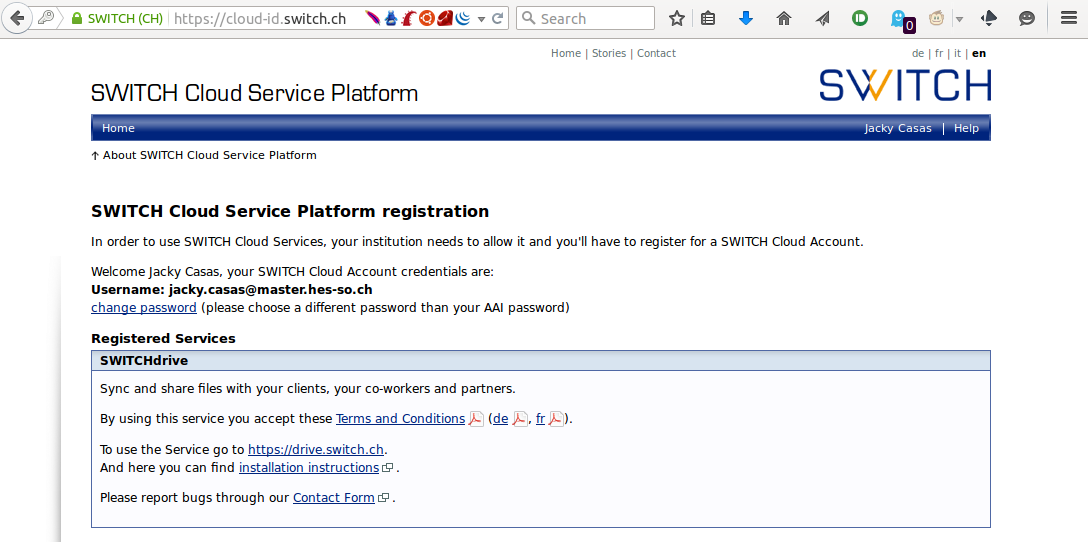
\includegraphics[width=\linewidth]{img/switch5.png}
  \caption{Récapitulatif, informations de votre compte}
  \label{enginesRecap}
\end{figure}

Sur cette figure, nous voyons que nous avons accès à SWITCHdrive (dans l'encadré), mais pas à SWITCHengines. Pour y avoir accès, il faut demander un accès en envoyant un e-mail à engines-support@switch.ch. Cette métodologie est valabe au moment de la rédaction de ce document. C'est pour faire partie de la phase pilote qui dure jusqu'à fin juin 2015.

%--> Users from academic can start using SWITCHengines as test users in the pilot phase of SWITCHengines. The pilot phase lasts until end of June 2015. Apply for an account on engines-support@switch.ch.
%\url{http://projects.switch.ch/scale/}

Vous recevrez un code d'activation par e-mail. Vous aurez ensuite accès à SWITCHengines, comme on le voit sur la figure \ref{enginesRecap2}.

\begin{figure}[h]
  \centering
    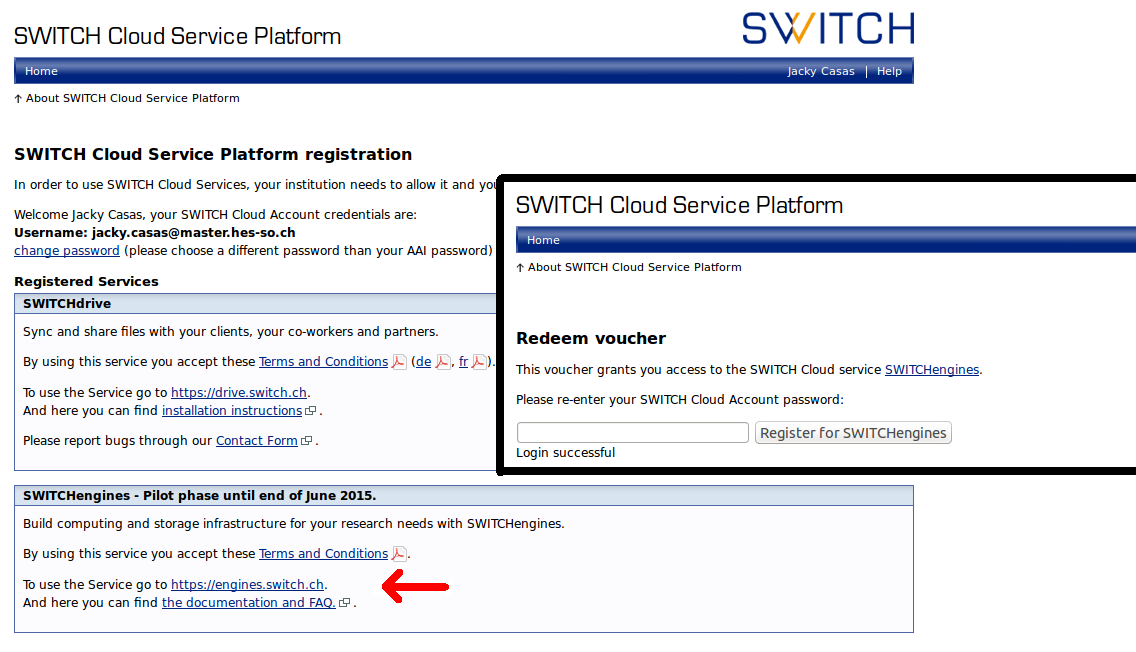
\includegraphics[width=\linewidth]{img/switch6.png}
  \caption{Accès à SWITCHengines et code d'activation}
  \label{enginesRecap2}
\end{figure}

\clearpage


%---------------------------------------------------------------------------------------------------------------------------------
\section{Connexion à SWITCHengines}


Si votre compte est configuré pour accéder à SWITCHengines, vous pouvez maintenant aller à l'adresse \url{https://engines.switch.ch/horizon} qui est la page de connexion (figure \ref{loginSWITCHengines}), et vous loguer.

\begin{figure}[h]
  \centering
    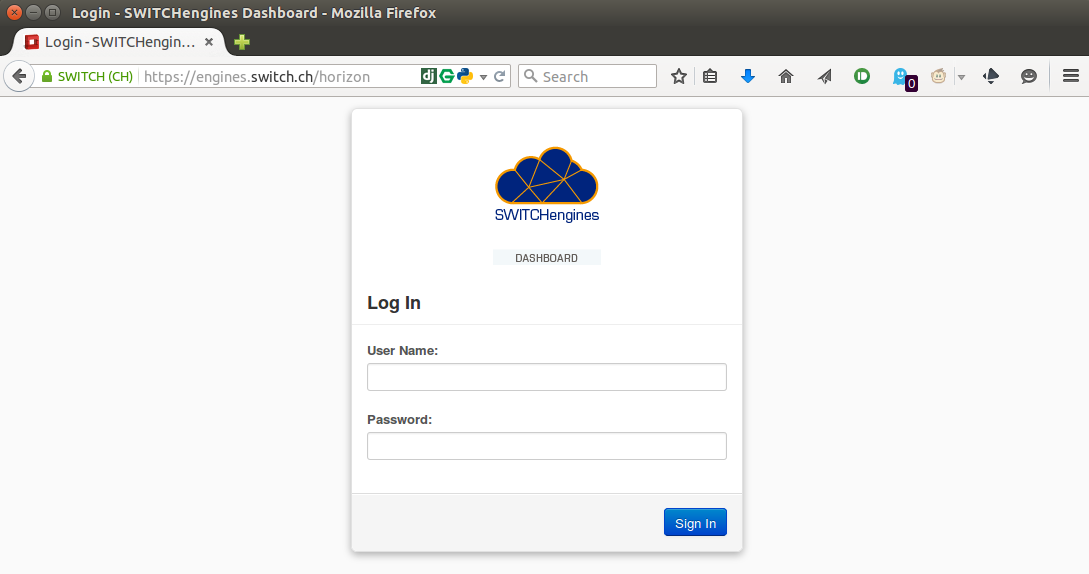
\includegraphics[width=\linewidth]{img/engines1.png}
  \caption{Page de connexion à SWITCHengines}
  \label{loginSWITCHengines}
\end{figure}

Vous arrivez ensuite sur le dashboard de SWITCHengines (figure \ref{dashboard1}). On voit sur l'image qu'aucune instance n'est pour l'instant créée. On va donc en créer une. 

\begin{figure}[h]
  \centering
    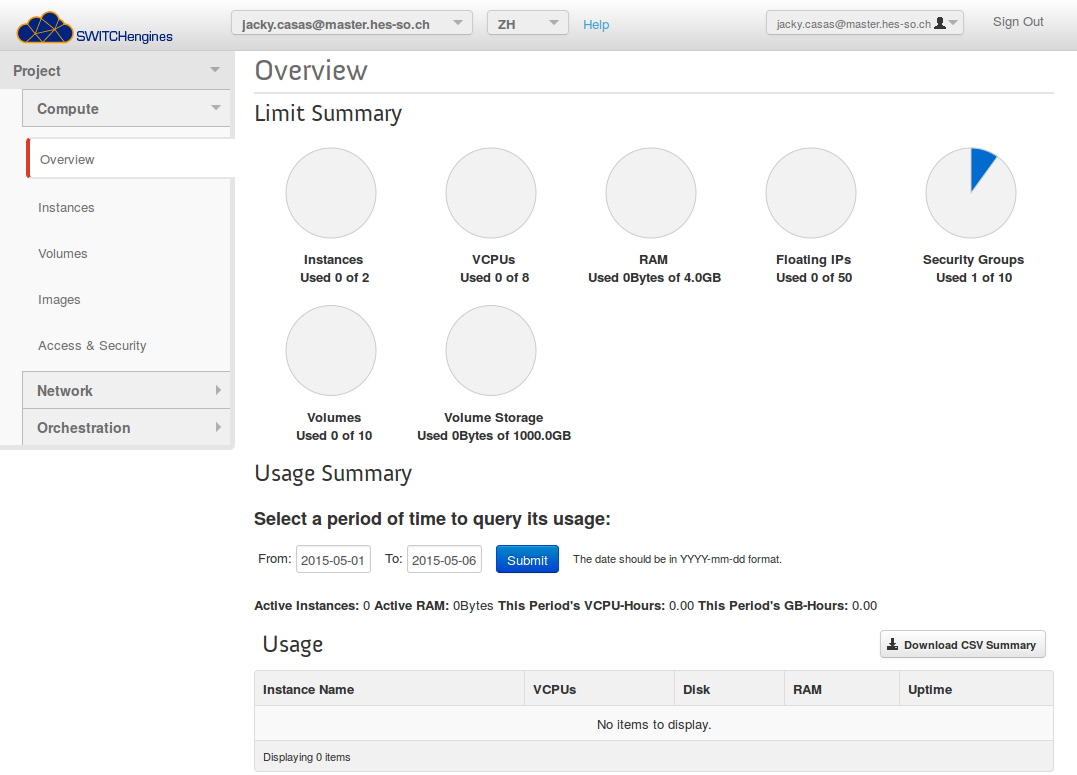
\includegraphics[width=\linewidth]{img/dashboard1.png}
  \caption{Dashboard de SWITCHengines}
  \label{dashboard1}
\end{figure}

\clearpage


%---------------------------------------------------------------------------------------------------------------------------------
\section{Création d'une instance}

\subsection{Choix de la zone}

Tout au sommet du dashboard se trouve un petit menu déroulant qui contient « ZH » et « LS ». Cela correspond à « Zürich » et « Lausanne ». Ce sont les deux zones disponibles, elles correspondent aux lieux où se trouvent les datacenters. Il faut choisir où on veut lancer notre instance avant de commencer.

\subsection{Création d'une paire de clés}

\begin{enumerate}
 \item Cliquer sur « Access \& Security » dans le menu de gauche.
 \item Cliquer sur l'onlet « Key Pairs ».
 \item Cliquer sur « + Create Key Pair ».
 \item Donner un nom à sa paire de clés.
 \item Télécharger le fichier .pem qui est la clé privée. Elle sera utilisée pour accéder aux instances créées.
\end{enumerate}


\subsection{Création d'un Security Group}

\begin{enumerate}
 \item Cliquer sur « Access \& Security » dans le menu de gauche.
 \item Cliquer sur le bouton « Manage Rules » à droite du Security Group par défaut. Cela va permettre d'éditer les règles d'accès.
 \item Cliquer sur « + Add Rule » pour ajouter une nouvelle règle.
 \item Choisir « SSH » dans le menu déroulant. Les champs suivants peuvent être laissés à leurs valeurs par défaut. Mais attention, si le CIDR est à 0.0.0.0/0, cela veut dire qu'on peut accéder à l'instance depuis n'importe où. Selon le but de l'instance, il faudrait limiter l'accès pour des raisons de sécurité.
 \item Cliquer sur « Add »  pour ajouter la règle. Nous pourrons donc accéder aux instances qui sont dans le Security Group par défaut par SSH.
\end{enumerate}

\noindent NB : pour pouvoir accéder à l'instance par HTTP ou HTTPS, il faut procéder de la même manière que pour ajouter la règle pour le SSH.
      
    
\subsection{Lancer une instance}

\begin{enumerate}
 \item Cliquer sur « Instances » dans le menu de gauche.
 \item Cliquer sur « Launch instance » en haut à droite.
 \item Donner un nom à l'instance, comme par exemple « owncloudserver ».
 \item Choisir la taille de l'instance, par exemple « c1.small ».
 \item Entrer 1 dans le nombre d'instance à lancer.
 \item Sélectionner « Boot from image » pour utiliser une image déjà existante d'un système d'exploitation.
 \item Choisir le système d'exploitation, par exemple « Ubuntu Trusty 14.04 (SWITCHengines) (1.5 GB) » pour une instance Ubuntu.
 \item Cliquer sur l'onglet « Access \& Security » et sélectionner la keypair créée précédemment
 \item Cliquer sur l'onglet « Networking » et sélectionner le réseau « private » (drag \& drop).
 \item Cliquer sur « Launch » en-bas à droite pour lancer l'instance. 
\end{enumerate}
    
\begin{figure}[h]
  \centering
    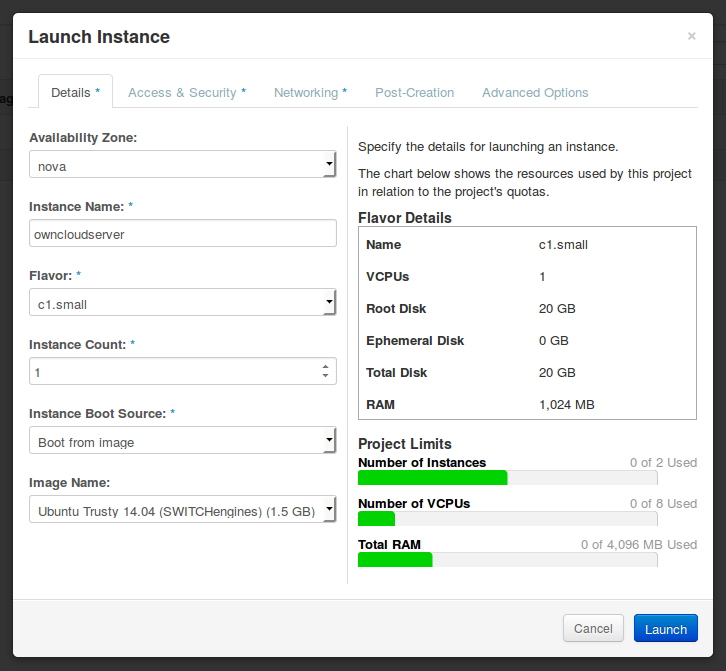
\includegraphics[width=0.7\linewidth]{img/instanceCreation1.png}
  \caption{Paramètres pour créer l'instance}
  \label{instanceCreation1}
\end{figure}

Si tout se passe bien, l'instance se lancer et elle est prête au bout de quelques secondes. Si au contraire ça ne fonctionne pas, il faut faire un tour sur les pages d'aide : \\
\url{https://help.switch.ch/engines}.

\subsection{Attribuer une IP flottante à l'instance}

Pour que l'instance ait une adresse IP accessible depuis internet (et pas uniquement depuis l'intérieur du cloud), il faut lui attribuer une IP. Pour ce faire, il faut aller à l'endroit où les instances sont listées et cliquer sur le bouton « More » (fig. \ref{instanceIP} point 1) puis « Associate Floating IP » (fig. \ref{instanceIP} point 2). Une fenêtre s'ouvre, vous devez sélectionner une IP. Si vous n'en avez pas, cliquer sur le petit « + » pour qu'une IP vous soit attribuée. Vous sélectionnez le port et cliquez sur « Associate ». Sur la liste des instances, vous pouvez maintenant voir que votre instance a une IP externe (fig. \ref{instanceIP} point 3).

\begin{figure}[h]
  \centering
    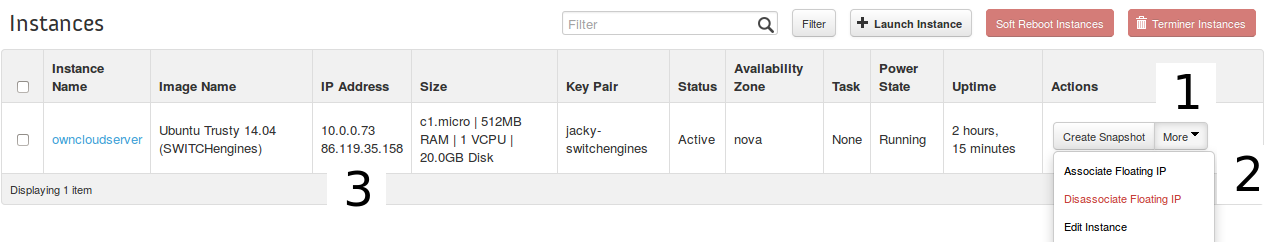
\includegraphics[width=\linewidth]{img/instanceIP.png}
  \caption{Etapes d'ajout d'une IP externe}
  \label{instanceIP}
\end{figure}

\subsection{Se connecter à l'instance}

Une fois l'instance lancée et l'IP attribuée, il est possible de se connecter à l'instance via SSH. Il faut aller à l'endroit où se trouve la clé privée précédemment créée et écrire la commande : ``\texttt{ssh -i <keypair.pem> <username>@<public IP>}'', où \texttt{<keypair.pem>} est la clé privée, \texttt{<username>} est le nom d'utilisateur créé pour l'instance (pour une instance ubuntu, le nom d'utilisateur est \texttt{ubuntu}, pour une instance CentOS, le nom d'utilisateur est \texttt{admin}) et \texttt{<public IP>} est l'IP public qu'on vient d'attribuer (dans ce cas, 86.119.35.158). \\

NB : si l'accès est refusé, c'est parce que les droits sur la clé privée sont trop laxistes, il faut donc restraintre les droits de cette manière : ``\texttt{sudo chmod 600 <keypair.pem>}'' 

NB2 : si ça ne fonctionne toujours pas, précédez la commande de connexion par ``\texttt{sudo}''

\vspace{0.6cm}
Voici la situation d'une connexion depuis un terminal standard :

\vspace{0.4cm}
\begin{lstlisting}[language=bash]
  jacky@grid:~$ ssh -i jacky-switchengines.pem ubuntu@86.119.35.158 
  Welcome to Ubuntu 14.04.2 LTS (GNU/Linux 3.13.0-48-generic x86_64)

  * Documentation:  https://help.ubuntu.com/

    System information as of Thu May 21 13:07:10 CEST 2015

    System load: 0.16              Memory usage: 10%   Processes:       51
    Usage of /:  65.5% of 1.30GB   Swap usage:   0%    Users logged in: 0

    Graph this data and manage this system at:
      https://landscape.canonical.com/

    Get cloud support with Ubuntu Advantage Cloud Guest:
      http://www.ubuntu.com/business/services/cloud

  0 packages can be updated.
  0 updates are security updates.


  The programs included with the Ubuntu system are free software;
  the exact distribution terms for each program are described in the
  individual files in /usr/share/doc/*/copyright.

  Ubuntu comes with ABSOLUTELY NO WARRANTY, to the extent permitted by
  applicable law.

  ubuntu@owncloudserver:~$
\end{lstlisting}

Pour se déconnecter de l'instance, il suffit juste d'écrire ``\texttt{exit}'' dans la console.
